%%%%%%%%%%%%%%%%%%%%%%%%%%%%%%%%%%%%%%%
% Deedy - One Page Two Column Resume
% LaTeX Template
% Version 1.2 (16/9/2014)
%
% Original author:
% Debarghya Das (http://debarghyadas.com)
%
% Original repository:
% https://github.com/deedydas/Deedy-Resume
%
% IMPORTANT: THIS TEMPLATE NEEDS TO BE COMPILED WITH XeLaTeX
%
% This template uses several fonts not included with Windows/Linux by
% default. If you get compilation errors saying a font is missing, find the line
% on which the font is used and either change it to a font included with your
% operating system or comment the line out to use the default font.
% 
%%%%%%%%%%%%%%%%%%%%%%%%%%%%%%%%%%%%%%
% 
% TODO:
% 1. Integrate biber/bibtex for article citation under publications.
% 2. Figure out a smoother way for the document to flow onto the next page.
% 3. Add styling information for a "Projects/Hacks" section.
% 4. Add location/address information
% 5. Merge OpenFont and MacFonts as a single sty with options.
% 
%%%%%%%%%%%%%%%%%%%%%%%%%%%%%%%%%%%%%%
%
% CHANGELOG:
% v1.1:
% 1. Fixed several compilation bugs with \renewcommand
% 2. Got Open-source fonts (Windows/Linux support)
% 3. Added Last Updated
% 4. Move Title styling into .sty
% 5. Commented .sty file.
%
%%%%%%%%%%%%%%%%%%%%%%%%%%%%%%%%%%%%%%%
%
% Known Issues:
% 1. Overflows onto second page if any column's contents are more than the
% vertical limit
% 2. Hacky space on the first bullet point on the second column.
%
%%%%%%%%%%%%%%%%%%%%%%%%%%%%%%%%%%%%%%


\documentclass[]{deedy-resume-openfont}
\usepackage{fancyhdr}
\usepackage{wrapfig}
\addtolength{\leftskip}{5em} \addtolength{\rightskip}{2em}
\pagestyle{fancy}
\fancyhf{}

\begin{document}

%%%%%%%%%%%%%%%%%%%%%%%%%%%%%%%%%%%%%%
%
%     LAST UPDATED DATE
%
%%%%%%%%%%%%%%%%%%%%%%%%%%%%%%%%%%%%%%

\lastupdated

%%%%%%%%%%%%%%%%%%%%%%%%%%%%%%%%%%%%%%
%
%     TITLE NAME
%
%%%%%%%%%%%%%%%%%%%%%%%%%%%%%%%%%%%%%%

\begin{wrapfigure}{l}{0.15\textwidth}\leftskip
    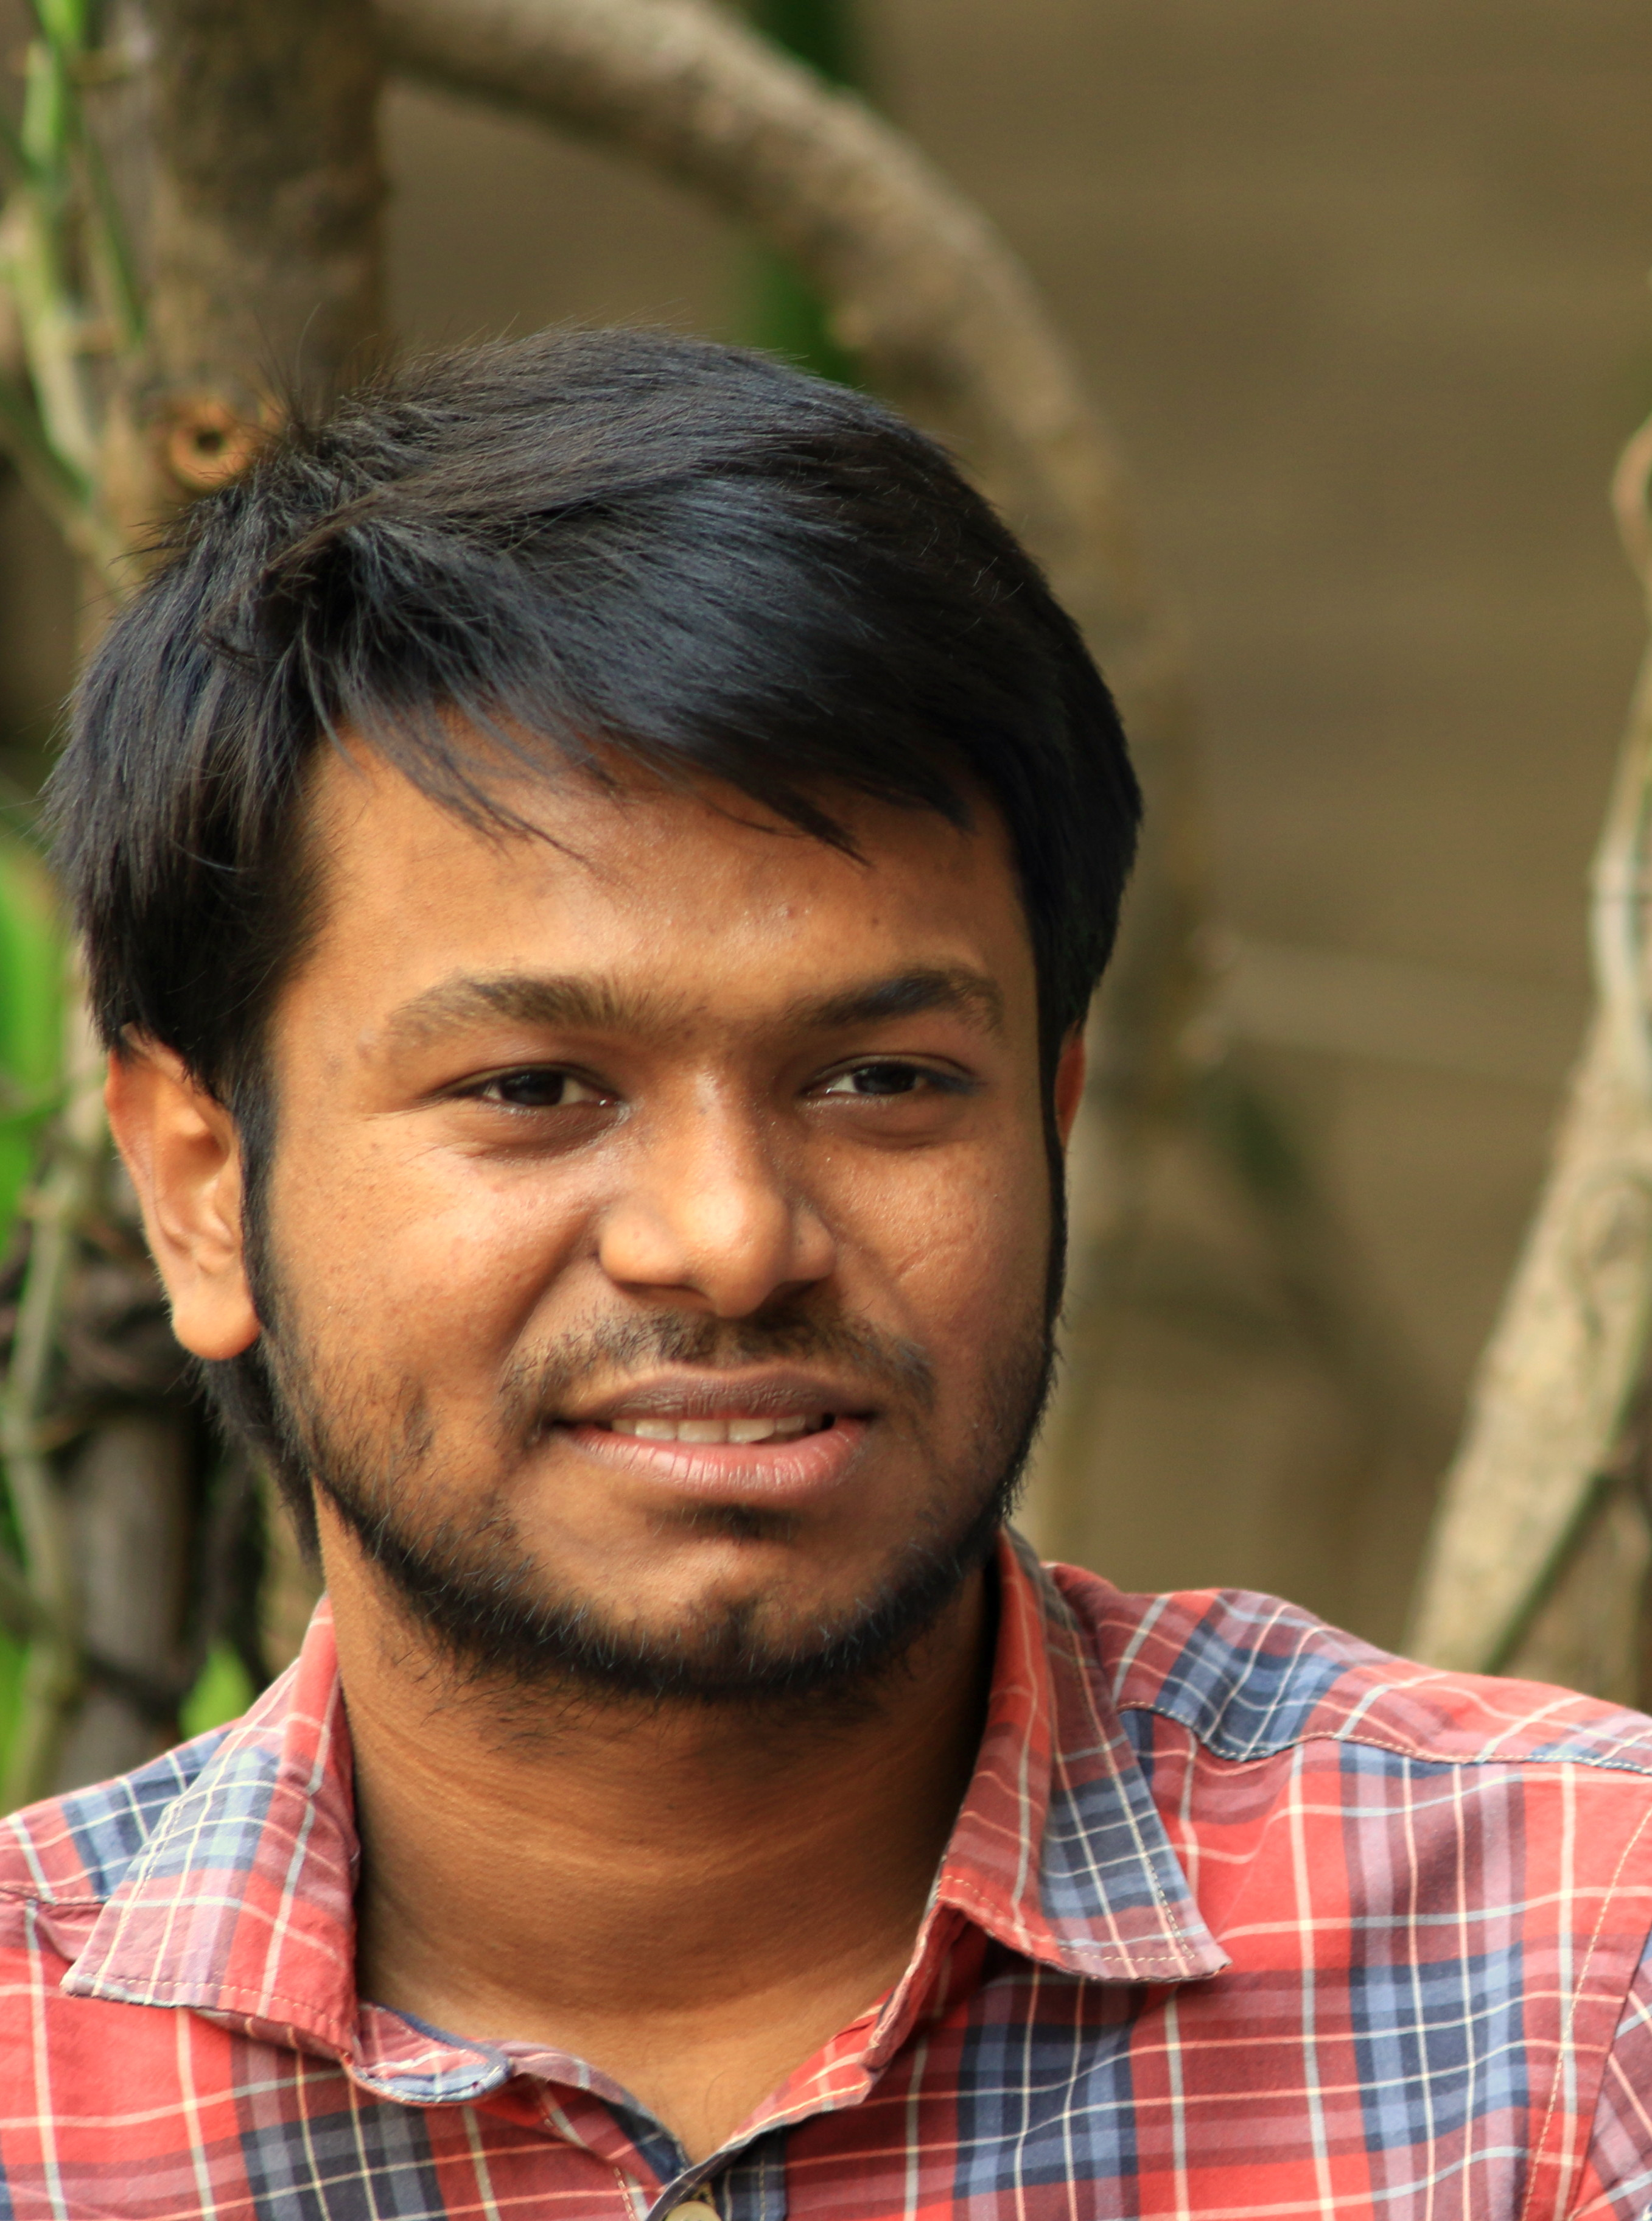
\includegraphics[width=2cm]{fonts/IMG_0666.JPG}
\end{wrapfigure}\\
\namesection{Nazmul Alam}{Diptu}{\\
\urlstyle{same}\href{https://github.com/diptu}{https://github.com/diptu}\\

\href{http://fb.com/nazmulalam.diptu}{fb.com/nazmulalam.diptu}\\
\href{mailto:nazmul.diptu@northsouth.edu}{ nazmul.diptu@northsouth.edu} | 01676133246 | \href{mailto:nazmul.diptu@northsouth.edu}{diptunazmulalam@gmail.com}
}


%%%%%%%%%%%%%%%%%%%%%%%%%%%%%%%%%%%%%%
%
%     COLUMN ONE
%
%%%%%%%%%%%%%%%%%%%%%%%%%%%%%%%%%%%%%%

\begin{minipage}[t]{0.33\textwidth} 

%%%%%%%%%%%%%%%%%%%%%%%%%%%%%%%%%%%%%%
%     EDUCATION
%%%%%%%%%%%%%%%%%%%%%%%%%%%%%%%%%%%%%%

\section{Education} 

% \subsection{Cornell University}
% \descript{MEng in Computer Science}
% \location{Dec 2014 | Ithaca, NY}
% \sectionsep

\subsection{North South University}
\descript{BS in Computer Science}
\location{Nov 2018 | Bashundhara \\ 
Dhaka, Bangladesh}
School of Engineering and Physical Sciences \\
Department of Electrical and Computer Engineering
\location{ Cum. GPA: 3.62 / 4.0 }
% Major GPA: 3.9 / 4.0}
\sectionsep

\subsection{Dhaka City College}
\location{HSC : Grad. May 2012|  Dhaka, Bangladesh}
\location{ GPA: 5.0 / 5.0 }
\sectionsep

\subsection{Ataturk Model High \\
School}
\location{SSC : Grad. April 2010|  Feni, Bangladesh}
\location{ GPA: 5.0 / 5.0 }
\sectionsep

%%%%%%%%%%%%%%%%%%%%%%%%%%%%%%%%%%%%%%
%     LINKS
%%%%%%%%%%%%%%%%%%%%%%%%%%%%%%%%%%%%%%

\section{Links} 
Facebook:// \href{https://facebook/nazmulalam.diptu}{\bf nazmulalam.diptu} \\
Github:// \href{https://github.com/diptu}{\bf diptu} \\
% LinkedIn://  \href{https://www.linkedin.com/in/debarghyadas}{\bf debarghyadas} 
Kaggle://  \href{https://www.kaggle.com/nazmulalamdiptu}{\bf nazmulalamdiptu} 
% Twitter://  \href{https://twitter.com/debarghya_das}{\bf @debarghya\_das} \\
% Quora://  \href{https://www.quora.com/Debarghya-Das}{\bf Debarghya-Das}

%%%%%%%%%%%%%%%%%%%%%%%%%%%%%%%%%%%%%%
%     COURSEWORK
%%%%%%%%%%%%%%%%%%%%%%%%%%%%%%%%%%%%%%

\section{Coursework}
\subsection{Undergraduate}
Machine Learning \\
Neural Networks \\
Theory of Fuzzy Systems \\
Internet and Web Technology \\
Concepts of Programming Language\\
Software Engineering \\
Operating Systems Design \\
Design and Analysis of Algorithms \\
Database Management System \\
Probability and Statistics \\
\sectionsep

% \subsection{Undergraduate}
% Information Retrieval \\
% Operating Systems \\
% Artificial Intelligence + Practicum \\
% Functional Programming \\
% Computer Graphics + Practicum \\
% {\footnotesize \textit{\textbf{(Research Asst. \& Teaching Asst 2x) }}} \\
% Unix Tools and Scripting \\

%%%%%%%%%%%%%%%%%%%%%%%%%%%%%%%%%%%%%%
%     SKILLS
%%%%%%%%%%%%%%%%%%%%%%%%%%%%%%%%%%%%%%

\section{Skills}
\subsection{Programming}
% \location{Over 5000 lines:}
Python \textbullet{} PHP \textbullet{} C \textbullet{}C++  \\
Java \textbullet{} Javascript \textbullet{} JQuery \textbullet{} SQL \\
Django \textbullet{} CodeIgniter \textbullet{} Laravel  \\ 

\location{Familiar:}
 \textbullet{} Matlab
\sectionsep

%%%%%%%%%%%%%%%%%%%%%%%%%%%%%%%%%%%%%%
%
%     COLUMN TWO
%
%%%%%%%%%%%%%%%%%%%%%%%%%%%%%%%%%%%%%%

\end{minipage} 
\hfill
\begin{minipage}[t]{0.66\textwidth} 

%%%%%%%%%%%%%%%%%%%%%%%%%%%%%%%%%%%%%%
%     EXPERIENCE
%%%%%%%%%%%%%%%%%%%%%%%%%%%%%%%%%%%%%%

\section{Experience}
\runsubsection{Academic | Personal}
\descript{|Hands on experience in project development and team management in multiple languages.}
\location{Jan 2015 - Present | Dhaka, Bangladesh}

\sectionsep
\section{Personal Summary}
\runsubsection{Personal objective}
\descript{| Currently i am looking for a software developer position or a Research assistant post in ML projects.}
\location{ I am a decent timekeeper, always arranged to learn new aptitudes. I am a quick learner. I am set up to work transparently in included conditions and in addition inside a social occasion setting. I am dynamic and sharp and arranged to listen enough when managing issues.I belief i am a quick learner.}

\sectionsep



% \runsubsection{Coursera}
% \descript{| KPCB Fellow + Software Engineering Intern }
% \location{June 2014 – Sep 2014 | Mountain View, CA}
% \vspace{\topsep} % Hacky fix for awkward extra vertical space
% \begin{tightemize}
% \item 52 out of 2500 applicants chosen to be a KPCB Fellow 2014.
% \item Led and shipped Yoda - the admin interface for the new Phoenix platform. 
% \item Full-stack developer - Wrote and reviewed code for JS using Backbone, Jade, Stylus and Require and Scala using Play
% \end{tightemize}
% \sectionsep

% \runsubsection{Google}
% \descript{| Software Engineering Intern }
% \location{May 2013 – Aug 2013 | Mountain View, CA}
% \begin{tightemize}
% \item Worked on the YouTube Captions team, in Javascript and Python to plan, to design and develop the full stack to add and edit Automatic Speech Recognition captions. In production.
% \item Created a backbone.js-like framework for the Captions editor.
% \end{tightemize}
% \sectionsep

% \runsubsection{Phabricator}
% \descript{| Open Source Contributor \& Team Leader}
% \location{Jan 2013 – May 2013 | Palo Alto, CA \& Ithaca, NY}
% \begin{tightemize}
% \item Phabricator is used daily by Facebook, Dropbox, Quora, Asana and more.
% \item I created the Meme generator and more in PHP and Shell.
% \item Led a team from MIT, Cornell, IC London and UHelsinki for the project.
% \end{tightemize}
% \sectionsep

%%%%%%%%%%%%%%%%%%%%%%%%%%%%%%%%%%%%%%
%     PUBLICATIONS
%%%%%%%%%%%%%%%%%%%%%%%%%%%%%%%%%%%%%%

\section{Publications} 
\renewcommand\refname{\vskip -1.5em} % Couldn't get this working from the .cls file
\bibliographystyle{abbrv}
\bibliography{publications}
\nocite{*}

\end{minipage} 
\end{document}  \documentclass[]{article}
